\documentclass[11pt,a4paper]{article}
\usepackage[a4paper,margin=1in]{geometry}
\usepackage{booktabs}
\usepackage{float}
\usepackage{graphicx}
\usepackage[hidelinks]{hyperref}

\title{U0-Anchor Multiple-Level Batch Gallery}
\author{}
\date{\today}

\begin{document}
\maketitle
\tableofcontents

\section*{Overview}
This note collects the multiple-level summary plots for the six benchmark cases
run with the paired schedule
\[
N = [2, 4, 6, 8, 10, 12, 14, 18], \qquad
p = [3, 5, 7, 9, 11, 13, 15, 19],
\]
with target continuation values $t = 10^{-p}$ at each level.

Each case section contains:
\begin{itemize}
  \item the summary plot \texttt{u0\_anchor\_multiple\_level\_error\_vs\_N.png},
  \item the per-level continuous-norm table extracted from the corresponding
  CSV summary file.
\end{itemize}

\section{Batch Summary}
\begin{table}[H]
  \centering
  \small
  \caption{Batch summary for the six multiple-level benchmark cases.}
  \resizebox{\textwidth}{!}{%
  \begin{tabular}{lrrrrrrrr}
    \toprule
    Case & Levels & Success & Final $N$ & Final $p$ & Final residual & Final ContL2 & Final ContH1 & CPU(s) \\
    \midrule
    \texttt{mild\_exp\_separable} & 8 & true & 18 & 19 & 5.760e-20 & 5.261e-15 & 5.621e-13 & 32.756 \\
    \texttt{mixed\_polynomial\_convex} & 8 & true & 18 & 19 & 5.551e-17 & 1.028e-14 & 1.122e-12 & 37.761 \\
    \texttt{mild\_sextic\_convex} & 8 & true & 18 & 19 & 1.041e-16 & 1.042e-14 & 1.136e-12 & 31.608 \\
    \texttt{gaussian\_bump\_convex} & 8 & true & 18 & 19 & 6.047e-16 & 5.177e-13 & 2.062e-11 & 38.346 \\
    \texttt{quartic\_convex} & 8 & true & 18 & 19 & 1.221e-15 & 2.597e-14 & 2.890e-12 & 30.603 \\
    \texttt{scaled\_quartic\_convex} & 8 & true & 18 & 19 & 2.776e-17 & 5.160e-15 & 5.786e-13 & 31.359 \\
    \bottomrule
  \end{tabular}}
\end{table}

\clearpage
\section{\texttt{mild\_exp\_separable}}
\begin{figure}[H]
  \centering
  
\includegraphics[width=0.88\textwidth]{../u0_anchor_monge_ampere_multiple_level_mild_exp_separable_demo_extended_8_levels/u0_anchor_multiple_level_error_vs_N.png}
  \caption{Multiple-level summary plot for \texttt{mild\_exp\_separable}.}
\end{figure}

\begin{table}[H]
  \centering
  \scriptsize
  \caption{Per-level summary for \texttt{mild\_exp\_separable}.}
  \begin{tabular}{rrrrrrrr}
    \toprule
    Level & $N$ & $p$ & start $t$ & target $t$ & ContL2 & ContH1 & CPU(s) \\
    \midrule
    1 & 2  & 3  & 1e+00 & 1e-03 & 1.055e-06 & 4.719e-06 & 4.144 \\
    2 & 4  & 5  & 1e-03 & 1e-05 & 1.305e-10 & 9.638e-10 & 4.070 \\
    3 & 6  & 7  & 1e-05 & 1e-07 & 2.042e-13 & 9.304e-13 & 4.059 \\
    4 & 8  & 9  & 1e-07 & 1e-09 & 3.629e-15 & 4.367e-14 & 3.913 \\
    5 & 10 & 11 & 1e-09 & 1e-11 & 3.629e-15 & 4.367e-14 & 3.761 \\
    6 & 12 & 13 & 1e-11 & 1e-13 & 3.629e-15 & 4.367e-14 & 4.367 \\
    7 & 14 & 15 & 1e-13 & 1e-15 & 3.629e-15 & 4.367e-14 & 4.118 \\
    8 & 18 & 19 & 1e-15 & 1e-19 & 5.261e-15 & 5.621e-13 & 4.323 \\
    \bottomrule
  \end{tabular}
\end{table}

\clearpage
\section{\texttt{mixed\_polynomial\_convex}}
\begin{figure}[H]
  \centering
  
\includegraphics[width=0.88\textwidth]{../u0_anchor_monge_ampere_multiple_level_mixed_polynomial_convex_demo_extended_8_levels/u0_anchor_multiple_level_error_vs_N.png}
  \caption{Multiple-level summary plot for \texttt{mixed\_polynomial\_convex}.}
\end{figure}

\begin{table}[H]
  \centering
  \scriptsize
  \caption{Per-level summary for \texttt{mixed\_polynomial\_convex}.}
  \begin{tabular}{rrrrrrrr}
    \toprule
    Level & $N$ & $p$ & start $t$ & target $t$ & ContL2 & ContH1 & CPU(s) \\
    \midrule
    1 & 2  & 3  & 1e+00 & 1e-03 & 6.025e-04 & 2.743e-03 & 4.300 \\
    2 & 4  & 5  & 1e-03 & 1e-05 & 1.164e-05 & 9.326e-05 & 4.072 \\
    3 & 6  & 7  & 1e-05 & 1e-07 & 2.522e-13 & 1.152e-12 & 4.186 \\
    4 & 8  & 9  & 1e-07 & 1e-09 & 6.271e-15 & 7.856e-14 & 4.279 \\
    5 & 10 & 11 & 1e-09 & 1e-11 & 2.767e-15 & 1.049e-13 & 3.934 \\
    6 & 12 & 13 & 1e-11 & 1e-13 & 2.136e-14 & 4.519e-13 & 3.886 \\
    7 & 14 & 15 & 1e-13 & 1e-15 & 4.377e-15 & 8.350e-14 & 5.305 \\
    8 & 18 & 19 & 1e-15 & 1e-19 & 1.028e-14 & 1.122e-12 & 7.800 \\
    \bottomrule
  \end{tabular}
\end{table}

\clearpage
\section{\texttt{mild\_sextic\_convex}}
\begin{figure}[H]
  \centering
  
\includegraphics[width=0.88\textwidth]{../u0_anchor_monge_ampere_multiple_level_mild_sextic_convex_demo_extended_8_levels/u0_anchor_multiple_level_error_vs_N.png}
  \caption{Multiple-level summary plot for \texttt{mild\_sextic\_convex}.}
\end{figure}

\begin{table}[H]
  \centering
  \scriptsize
  \caption{Per-level summary for \texttt{mild\_sextic\_convex}.}
  \begin{tabular}{rrrrrrrr}
    \toprule
    Level & $N$ & $p$ & start $t$ & target $t$ & ContL2 & ContH1 & CPU(s) \\
    \midrule
    1 & 2  & 3  & 1e+00 & 1e-03 & 1.197e-03 & 5.450e-03 & 3.795 \\
    2 & 4  & 5  & 1e-03 & 1e-05 & 2.322e-05 & 1.863e-04 & 3.722 \\
    3 & 6  & 7  & 1e-05 & 1e-07 & 9.583e-13 & 4.356e-12 & 3.604 \\
    4 & 8  & 9  & 1e-07 & 1e-09 & 1.299e-14 & 9.582e-14 & 3.817 \\
    5 & 10 & 11 & 1e-09 & 1e-11 & 2.819e-15 & 1.057e-13 & 3.908 \\
    6 & 12 & 13 & 1e-11 & 1e-13 & 2.162e-14 & 4.594e-13 & 4.061 \\
    7 & 14 & 15 & 1e-13 & 1e-15 & 4.309e-15 & 8.486e-14 & 4.477 \\
    8 & 18 & 19 & 1e-15 & 1e-19 & 1.042e-14 & 1.136e-12 & 4.224 \\
    \bottomrule
  \end{tabular}
\end{table}

\clearpage
\section{\texttt{gaussian\_bump\_convex}}
\begin{figure}[H]
  \centering
  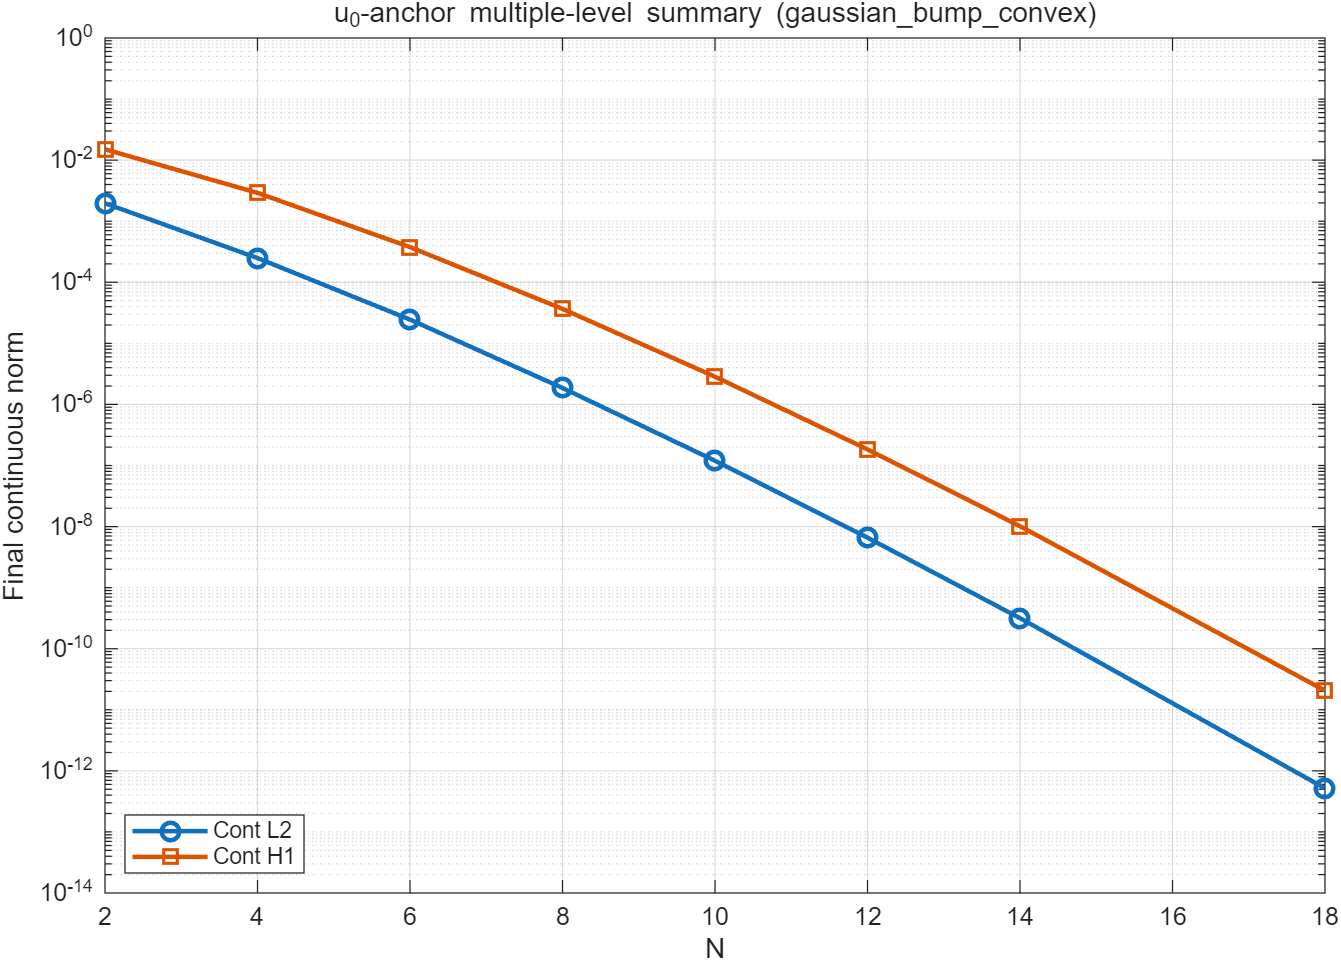
\includegraphics[width=0.88\textwidth]{../u0_anchor_monge_ampere_multiple_level_gaussian_bump_convex_demo_extended_8_levels/u0_anchor_multiple_level_error_vs_N.png}
  \caption{Multiple-level summary plot for \texttt{gaussian\_bump\_convex}.}
\end{figure}

\begin{table}[H]
  \centering
  \scriptsize
  \caption{Per-level summary for \texttt{gaussian\_bump\_convex}.}
  \begin{tabular}{rrrrrrrr}
    \toprule
    Level & $N$ & $p$ & start $t$ & target $t$ & ContL2 & ContH1 & CPU(s) \\
    \midrule
    1 & 2  & 3  & 1e+00 & 1e-03 & 1.967e-03 & 1.505e-02 & 4.756 \\
    2 & 4  & 5  & 1e-03 & 1e-05 & 2.492e-04 & 2.910e-03 & 4.064 \\
    3 & 6  & 7  & 1e-05 & 1e-07 & 2.452e-05 & 3.771e-04 & 3.823 \\
    4 & 8  & 9  & 1e-07 & 1e-09 & 1.860e-06 & 3.665e-05 & 3.796 \\
    5 & 10 & 11 & 1e-09 & 1e-11 & 1.196e-07 & 2.846e-06 & 10.226 \\
    6 & 12 & 13 & 1e-11 & 1e-13 & 6.579e-09 & 1.838e-07 & 3.763 \\
    7 & 14 & 15 & 1e-13 & 1e-15 & 3.168e-10 & 1.016e-08 & 3.692 \\
    8 & 18 & 19 & 1e-15 & 1e-19 & 5.177e-13 & 2.062e-11 & 4.225 \\
    \bottomrule
  \end{tabular}
\end{table}

\clearpage
\section{\texttt{quartic\_convex}}
\begin{figure}[H]
  \centering
  
\includegraphics[width=0.88\textwidth]{../u0_anchor_monge_ampere_multiple_level_quartic_convex_demo_extended_8_levels/u0_anchor_multiple_level_error_vs_N.png}
  \caption{Multiple-level summary plot for \texttt{quartic\_convex}.}
\end{figure}

\begin{table}[H]
  \centering
  \scriptsize
  \caption{Per-level summary for \texttt{quartic\_convex}.}
  \begin{tabular}{rrrrrrrr}
    \toprule
    Level & $N$ & $p$ & start $t$ & target $t$ & ContL2 & ContH1 & CPU(s) \\
    \midrule
    1 & 2  & 3  & 1e+00 & 1e-03 & 1.403e-02 & 6.309e-02 & 3.628 \\
    2 & 4  & 5  & 1e-03 & 1e-05 & 6.416e-15 & 7.569e-14 & 3.570 \\
    3 & 6  & 7  & 1e-05 & 1e-07 & 1.382e-14 & 1.747e-13 & 4.012 \\
    4 & 8  & 9  & 1e-07 & 1e-09 & 1.134e-14 & 1.908e-13 & 3.968 \\
    5 & 10 & 11 & 1e-09 & 1e-11 & 7.239e-15 & 2.794e-13 & 4.320 \\
    6 & 12 & 13 & 1e-11 & 1e-13 & 5.277e-14 & 1.213e-12 & 3.732 \\
    7 & 14 & 15 & 1e-13 & 1e-15 & 9.733e-15 & 2.042e-13 & 3.715 \\
    8 & 18 & 19 & 1e-15 & 1e-19 & 2.597e-14 & 2.890e-12 & 3.658 \\
    \bottomrule
  \end{tabular}
\end{table}

\clearpage
\section{\texttt{scaled\_quartic\_convex}}
\begin{figure}[H]
  \centering
  
\includegraphics[width=0.88\textwidth]{../u0_anchor_monge_ampere_multiple_level_scaled_quartic_convex_demo_extended_8_levels/u0_anchor_multiple_level_error_vs_N.png}
  \caption{Multiple-level summary plot for \texttt{scaled\_quartic\_convex}.}
\end{figure}

\begin{table}[H]
  \centering
  \scriptsize
  \caption{Per-level summary for \texttt{scaled\_quartic\_convex}.}
  \begin{tabular}{rrrrrrrr}
    \toprule
    Level & $N$ & $p$ & start $t$ & target $t$ & ContL2 & ContH1 & CPU(s) \\
    \midrule
    1 & 2  & 3  & 1e+00 & 1e-03 & 2.807e-03 & 1.262e-02 & 3.790 \\
    2 & 4  & 5  & 1e-03 & 1e-05 & 3.835e-09 & 1.727e-08 & 4.073 \\
    3 & 6  & 7  & 1e-05 & 1e-07 & 3.835e-11 & 1.727e-10 & 3.862 \\
    4 & 8  & 9  & 1e-07 & 1e-09 & 3.849e-13 & 1.734e-12 & 3.965 \\
    5 & 10 & 11 & 1e-09 & 1e-11 & 4.324e-15 & 5.976e-14 & 3.909 \\
    6 & 12 & 13 & 1e-11 & 1e-13 & 1.073e-14 & 2.442e-13 & 3.782 \\
    7 & 14 & 15 & 1e-13 & 1e-15 & 2.025e-15 & 4.232e-14 & 3.837 \\
    8 & 18 & 19 & 1e-15 & 1e-19 & 5.160e-15 & 5.786e-13 & 4.141 \\
    \bottomrule
  \end{tabular}
\end{table}

\end{document}
